%% LyX 2.2.3 created this file.  For more info, see http://www.lyx.org/.
%% Do not edit unless you really know what you are doing.
\documentclass[DM,lsstdraft,toc,authoryear]{lsstdoc}
\usepackage{prettyref}

\makeatletter

%%%%%%%%%%%%%%%%%%%%%%%%%%%%%% LyX specific LaTeX commands.

\title[jointcal]{jointcal: Simultaneous Astrometry \& Photometry for thousands of
Exposures with Large CCD Mosaics}
\author{John Parejko (University of Washington), Pierre Astier (LPNHE/IN2P3/CNRS
Paris)}
\setDocRef{DMTN-036}
\date{2017-09-18}
\setDocAbstract{The jointcal package simultaneously optimizes the astrometric and
photometric calibrations of a set of astronomical images. In principle
and often in practice, this approach produces distortion and thoroughput
models which are more precise than when fitted independently. This
is especially true when the images are deeper than the astrometric
reference catalogs. In the ``Astromatic'' software suite, this simultaneous
astrometry functionality is fulfilled by ``SCAMP''. The code we
describe here has similar aims, but follows a slightly different route.
Jointcal is built on top of the the LSST Data Management software
stack.}

%%%%%%%%%%%%%%%%%%%%%%%%%%%%%% User specified LaTeX commands.
% Change history defined here.
% Order: oldest first.
% Fields: VERSION, DATE, DESCRIPTION, OWNER NAME.
% See LPM-51 for version number policy.
\setDocChangeRecord{%
  \addtohist{1}{2017-09-18}{Initial release. Moved from jointcal repo.}{John Parejko}
}

\makeatother

\usepackage{xunicode}
\begin{document}
\maketitle

\section{Introduction}

With deep astronomical images, it is extremely common that the relative
astrometry and photometry between images is considerably more precise
than the accuracy of external catalogs, where ``more precise'' can
be as large as two orders of magnitude. For applications where the
quality of relative astrometry is important or vital, it is important
to rely on some sort of simultaneous astrometry solution, if possible
optimal in a statistical sense.

This package performs a least-squares fit to a set of images. Since
it aims at statistical optimality, we maximize the likelihood of the
measurements with respect to all unknown parameters required to describe
the data. These parameters are mostly in two sets: the position on
the sky of the objects in common between the images, and the mapping
of each image to the sky. To these obvious parameters, one can add
proper motions (where applicable), and parameters describing the differential
effect of atmospheric refraction on the position of objects. It is
clear that one cannot fit simultaneously the position on the sky and
the mappings from CCD coordinates to the sky, without extra constraints:
the ``sky'' coordinate system is then undefined, and one needs reference
positions in order to fully define this frame. We use the GAIA catalog
\citep{2016A&A...595A...2G} as our reference catalog, and may supplement
it with deeper data (e.g. PS1) where available.

SCAMP \citep{2006ASPC..351..112B} is the reference package for simultaneous
astrometry in astronomy, at least for relative alignment of wide-field
images prior to stacking. Regarding optimization, SCAMP follows a
somewhat different route from ours: it does not optimize over the
position of common objects but rather minimizes the distance between
pairs of transformed measurements of the same object. This approach
is not a maximum likelihood optimization, and is likely statistically
sub-optimal. The main drawback of SCAMP in the context of LSST is
the fact that it is a program and not a library, and hence not flexible
regarding formats of images and catalogs. But since SCAMP has been
used for almost a decade in production by various teams, the quality
checking tools it provides should likely be reproduced in the context
of our package. We provide residual ntuples and hope that the first
serious users will contribute plotting tools.

Loading input catalogs and their metadata from disk is a large fraction
of the total time. We can save time by re-using the input catalog
to fit a similar style of multi-component model for the relative and
absolute photometry.

The plan of this note is as follows: we first sketch the algorithm
(\prettyref{sec:algo}). We provide our least-squares formulation
in \prettyref{sec:mathematical-formalism}, and describe the how we
evaluate the derivatives with respect to the parameters. We then describe
how we associate the measurements of each object in different exposures
in \prettyref{sec:catalog-association}. 

\section{Past work}

A summary of past work on this topic will go here eventually...
\begin{itemize}
\item Photographic Plates \citep{1960AN....285..233E}
\item SDSS übercal \citep{2008ApJ...674.1217P}
\item Pan-Starrs übercal \citep{2013ApJS..205...20M}
\item DECam WcsFit \citep{2017PASP..129g4503B}
\end{itemize}

\section{Algorithm flow \label{sec:algo}}

The algorithm assumes that the initial single-frame WCS fits of the
input images are accurate to $\sim1\arcsec$. Currently, the code
properly interprets the SIP WCS's (relying on \code{lsst::afw::wcs}),
with or without distortions. The code might handle transparently the
``PV'' encoding of distortions (used in SCAMP and Swarp), but lacks
the IO's required to use this format. Note that in both instances,
the WCS boils down to a polynomial 2D transform from CCD space to
a tangent plane, followed by a gnomonic de-projection to the celestial
sphere. The difference between formats lies into the encoding of the
polynomial, but they map exactly the same space of distortion functions.

The algorithm can be roughly split into these successive steps: 
\begin{enumerate}
\item load the input catalogs and 'rough' WCS's and catalogs, and select
the sources to use in the fit (e.g. good centroids, unblended, high
enough signal-to-noise) via the configured SourceSelectorTask.
\item Associate these catalogs, i.e. associate each detection of the same
on-sky source, and associate those on-sky sources with a reference
catalog (if provided).
\item Iteratively fit the model parameters and ``true'' on-sky values,
clipping outliers at each iteration.
\item Output results. 
\end{enumerate}

\section{Mathematical formalism\label{sec:mathematical-formalism}}

\subsection{Definitions\label{subsec:Definitions}}

\begin{figure*}
\begin{centering}
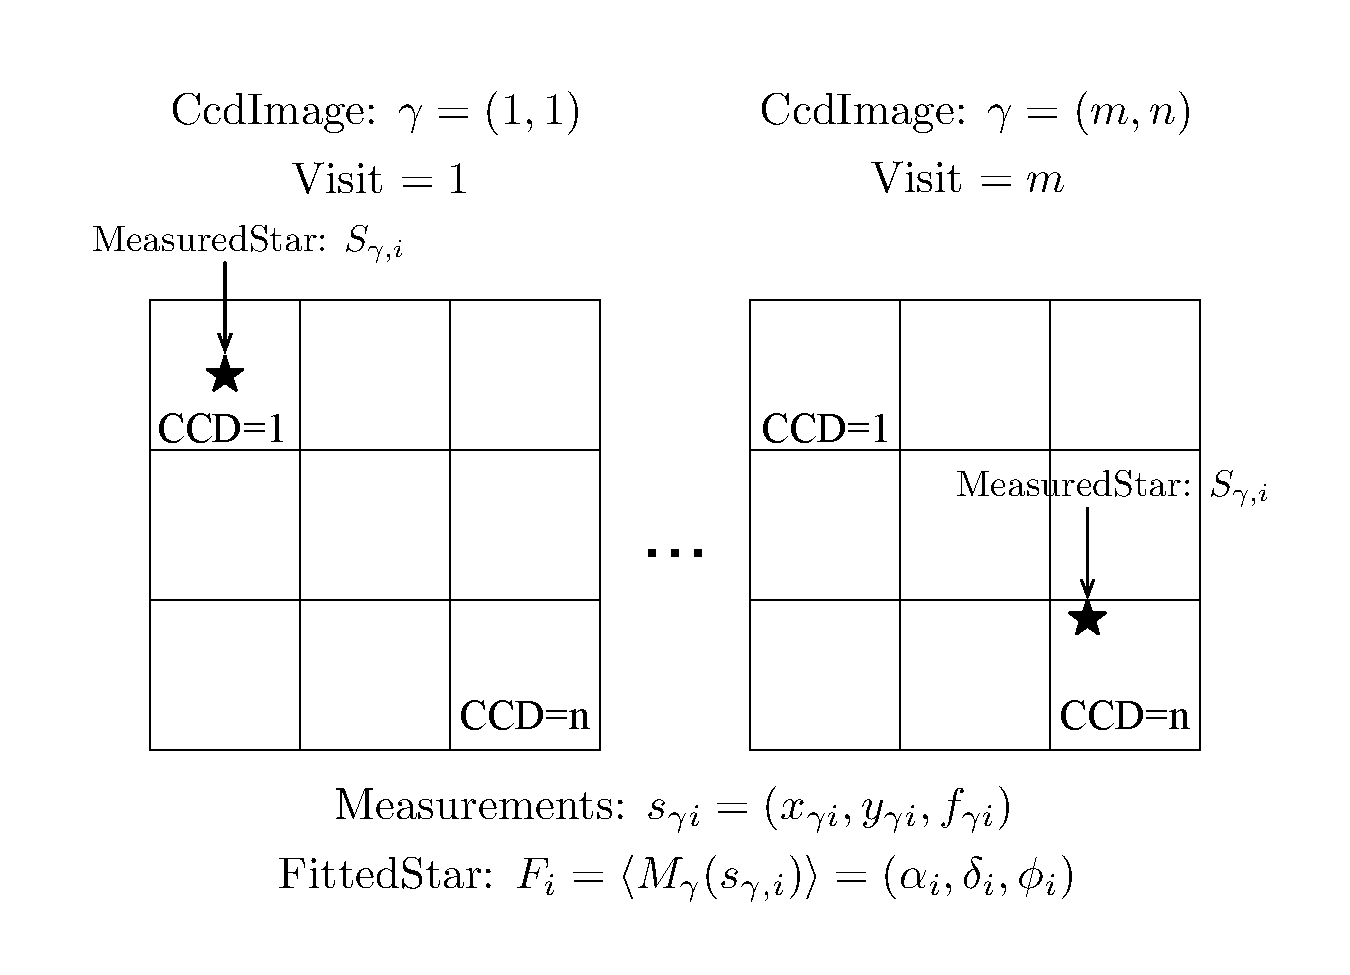
\includegraphics[width=0.8\textwidth]{_static/CcdImageDiagram}
\par\end{centering}
\caption{The relationship between MeasuredStars, CcdImages, and FittedStars.\label{fig:NotationDigram}}
\end{figure*}

We use the following notation in the mathematics that follows, with
\class{CamelCased} words referring to the objects in the code. These
terms are diagramed in \prettyref{fig:NotationDigram}.
\begin{itemize}
\item $\gamma$ is the \class{CcdImage} representing one exposure (\emph{visit}
in LSST terminology) on one CCD. The \class{CcdImage} contains metadata
about that visit and CCD detector, as well as the catalog of sources
that were selected for use in the fit;
\item $S_{\gamma,i}$ is the position (pixels) and flux (instrument-flux
counts) ($x_{\gamma i},y_{\gamma i},f_{\gamma i}$) of the \class{MeasuredStar}
on \class{CcdImage} $\gamma$ corresponding to the on-sky \class{FittedStar}
$i$;
\item $F_{i}$ is the (sky) position and calibrated-flux $(\alpha_{i},\beta_{i},\phi_{i})$
of the star $i$, with some corresponding number of measurements represented
by \class{MeasuredStar}s;
\item $M_{\gamma}$ is the mapping for \class{CcdImage} $\gamma$ from
pixels/instrument-flux $(x,y,f)$ to the tangent plane on the sky/calibrated-flux
$(\alpha,\beta,\phi)$. This mapping may consist of models constrained
across visits (different between CCDs; e.g. an affine model for each
CCD position, assuming CCDs do not move), constrained across CCDs
and visits (e.g. a 2d radial polynomial of the optics) or constrained
across CCDs (different between visits; e.g. a 2d polynomial of the
sky);
\item $R_{j}$ refers to the (sky) position and (reference) calibrated-flux
$(\alpha_{j},\beta_{j},\phi_{j})$ of \class{RefStar} $j$.
\end{itemize}
In addition to the terms defined in the diagram above, we define the
following terms for the measurement component,
\begin{itemize}
\item $P_{\gamma}$ is a projector from sidereal coordinate to some tangent
plane; $P_{\gamma}$ is user-defined;
\item $W_{\gamma,i}$ is the measurement weight of $M_{\gamma}(S_{\gamma,i})$,
i.e. the inverse of the 2$\times$2 covariance matrix (for astrometry),
or the inverse of the transformed instrument-flux error;
\end{itemize}
and reference component, 
\begin{itemize}
\item $P$ is some (user-provided) sky to tangent plane projector;
\item $W_{j}$ is the weight matrix of the reference star, i.e. the inverse
of the projected position error $P(R_{j})$, or the inverse of the
reference flux error.
\end{itemize}

\subsection{Least-squares expression}

The fit consists of minimizing, for photometry, 
\begin{align}
\chi^{2} & =\sum_{\gamma,i}[M_{\gamma}(S_{\gamma,i})-F_{i}]^{T}W_{\gamma,i}[M_{\gamma}(S_{\gamma,i})-F_{i}] & \textrm{(meas. terms)}\nonumber \\
 & +\sum_{j}[F_{j}-R_{j}]^{T}W_{j}[F_{j}-R_{j}] & \textrm{(ref. terms)}\label{eq:photometry-chi2}
\end{align}
and for astrometry, taking into account the projection from the sky
to the tangent plane $P$:
\begin{align}
\chi^{2} & =\sum_{\gamma,i}[M_{\gamma}(S_{\gamma,i})-P_{\gamma}(F_{i})]^{T}W_{\gamma,i}[M_{\gamma}(S_{\gamma,i})-P_{\gamma}(F_{i})] & \textrm{(meas. terms)}\nonumber \\
 & +\sum_{j}[P(F_{j})-P(R_{j})]^{T}W_{j}[P(F_{j})-P(R_{j})] & \textrm{(ref. terms)}\label{eq:astrometry-chi2}
\end{align}
where the first line iterates on all \class{MeasuredStar} $\gamma,i$,
from all \class{CcdImage} $\gamma$, and the second iterates on all
\class{RefStar} $j$. In the first terms, the object at position
$F_{i}$ is the one that was measured at position $S_{\gamma,i}$
in image $\gamma$. The association between \class{MeasuredStar}s,
\class{FittedStar}s, and \class{RefStar}s is described in \prettyref{sec:catalog-association}.

The measurement terms compare the measurement positions/fluxes to
objects positions/fluxes (the relative astrometry/photometry), the
reference terms compare object positions/fluxes to reference positions/fluxes
(the absolute astrometry/photometry). We need these two sets of terms
because not all objects $F_{i}$ in the first terms appear in the
second terms: many objects in the images will not be in the reference
catalogs, but those objects do help to constrain the mappings $M_{\gamma}$.
In addition, with so many measurements of our sources, we may have
better overall errors on the positions and fluxes than the reference
catalog can provide.

The expressions above depend on two sets of parameters: the parameters
defining the mappings $M$ and the on-sky positions/calibrated fluxes
$F_{i}$. For a practical problem, this amounts to a very large number
of parameters, which becomes tractable when one notes that every term
in the $\chi2$ is only linked to a small number of parameters. We
exploit this feature to rapidly compute the gradient and the Hessian
of the $\chi^{2}$ in order to find the minimum.

So far, we have not specified how we model the mappings $M$ nor how
we choose the various projectors that appear in expression \prettyref{eq:astrometry-chi2}.
The code has been written to allow the user to provide their own versions
of both the model for mappings and the projection scheme. We however
provide some implementations for both aspects that we discuss in the
next two sections.

\subsection{Minimization approach}

The expressions for astrometry (eq. \prettyref{eq:astrometry-chi2})
and photometry (eq. \prettyref{eq:photometry-chi2}) depend on two
sets of parameters: the parameters $\eta$ defining the mappings $M_{\gamma}(S_{\gamma,i})\equiv M_{\gamma}(\eta_{\gamma},S_{\gamma,i})$,
and the ``true'' calibrated fluxes $F_{i}$. We write the measurement
and reference residuals, with their respective weights $W_{\gamma i}$
and $W_{j}$, as separate functions of their parameters, for photometry,

\begin{align}
D_{\gamma i} & =M_{\gamma}(S_{\gamma,i})-F_{i}\label{eq:photometry_residual_vector_measurement}\\
D_{j} & =F_{j}-R_{j}\label{eq:photometry_residual_vector_reference}
\end{align}
and for astrometry,

\begin{align}
D_{\gamma i} & =M_{\gamma}(S_{\gamma,i})-P_{\gamma}(F_{i})\label{eq:astrometry_residual_vector_measurement}\\
D_{j} & =[P(F_{j})-P(R_{j})]\label{eq:astrometry_residual_vector_reference}
\end{align}
This results in the generalized $\chi^{2}$ expression (compare to
eq. \prettyref{eq:astrometry-chi2} and \prettyref{eq:photometry-chi2}),

\begin{align}
\chi^{2} & =\sum_{\gamma,i}{D_{\gamma i}}^{T}W_{\gamma,i}D_{\gamma i}\nonumber \\
 & +\sum_{j}{D_{j}}^{T}W_{j}D_{j}\label{eq:chi2-with-residuals}
\end{align}
To minimize this $\chi^{2}$, we want to find the point in parameter
space where the gradient $\nabla\chi^{2}=d\chi^{2}/d\theta=0$, where
$\theta$ denotes the vector of parameters (of size $N_{p}$– see
below). Applying the product rule and noting the symmetry of $D$
and $D^{T}$, we have
\begin{align}
\frac{1}{2}\frac{d\chi^{2}}{d\theta} & =\sum_{\gamma,i}{D_{\gamma i}}^{T}W_{\gamma,i}\nabla D_{\gamma i}\nonumber \\
 & +\sum_{j}{D_{j}}^{T}W_{j}\nabla D_{j}\label{eq:def_chi2_gradient}
\end{align}
where the $\nabla D$ matrices have size $2\times N_{p}$ (for astrometry)
and $1\times N_{p}$ (for photometry):
\begin{align}
\nabla D_{\gamma i} & =\frac{d{D_{\gamma i}}}{d\theta}\\
\nabla D_{j} & =\frac{d{D_{j}}}{d\theta}
\end{align}

We call the vector that gathers all the parameters to be fit during
the minimization $\theta=(\eta_{\gamma},F_{i})$. This vector can
easily exceed $N_{p}>10^{5}$ entries. As an example with LSST (having
a 189-CCD camera), a mapping consisting of a 3rd order 2-D polynomial
per visit (16 $\eta_{k}$ parameters per visit) and 100 viable sources
per CCD with 15 visits (roughly a year of LSST observations of one
sky location in one filter), $\theta$ will have $N_{p}=283,740$
entries ($283,500$ $F_{i}$ parameters + $240$ model parameters).
However, the second derivative matrix, $d^{2}\chi^{2}/d\theta^{2}$,
is very sparse, because there are no terms connecting $F_{i}$ and
$F_{j}$ if $i\neq j$, and depending on how the mappings are parametrized,
a set of $\eta_{\gamma}$ parameters could be connected (in the second
derivative matrix) to only a small set of $F_{j}$'s. So, we can search
for the minimum $\chi^{2}$ using methods involving the second derivative
matrix, taking advantage of its sparseness.

We are looking for the offset to the starting parameters that zeros
the gradient, so we can Taylor expand about that starting parameter
vector $\theta_{0}$,

\[
0=\frac{d\chi^{2}}{d\theta}(\theta_{0}+\delta\theta)=\frac{d\chi^{2}}{d\theta}(\theta_{0})+\frac{d^{2}\chi^{2}}{d\theta^{2}}(\theta_{0})\delta\theta+O(\delta\theta^{2})
\]
and solve for the offset $\delta\theta$ that zeroes it to first order,
\begin{eqnarray}
\left[\frac{d^{2}\chi^{2}}{d\theta^{2}}(\theta_{0})\right]\delta\theta & = & -\frac{d\chi^{2}}{d\theta}(\theta_{0})\label{eq:step_definition}\\
H\delta\theta & = & -\nabla\chi^{2}\label{eq:hessian_step}
\end{eqnarray}
where we have identified the second derivative matrix with the Hessian
matrix $H$. Working from eq. \prettyref{eq:def_chi2_gradient}, we
can write the second derivative matrix (the Hessian) as:
\begin{align}
\frac{1}{2}\frac{d^{2}\chi^{2}}{d\theta^{2}} & =\sum_{\gamma,i}{\nabla D_{\gamma i}}^{T}W_{\gamma,i}\nabla D_{\gamma i}\nonumber \\
 & +\sum_{j}{\nabla D_{j}}^{T}W_{j}\nabla D_{j}\label{eq:def_hessian}
\end{align}
where we have neglected the second derivatives of the residual vectors
$D$. This second derivative matrix is by construction symmetric,
and hence the parameter offsets (defined in eq. \prettyref{eq:step_definition})
can be evaluated using the (fast) Cholesky $LDL^{T}$ factorization
(see \prettyref{subsec:linear-solver-note}). If possible, mappings
$M_{\gamma}(\eta_{\gamma},S)$ linear with respect to their parameters
$\eta_{\gamma}$, for example polynomials, are to be favored because
the second derivatives will no longer depend on that parameter. If
the problem were non-linear (more precisely, if the second derivative
varies rapidly) we would have to implement a line search to minimize
$\chi^{2}(\theta_{0}+\lambda\times\delta\theta)$ over $\lambda$.

Returning to the weights, we note that the matrices $W_{\gamma,i}$
are positive-definite and thus they have square roots (e.g. the Cholesky
square root) and can be written as: $W_{\gamma,i}=\alpha_{\gamma i}^{T}\alpha_{\gamma i}$.
Defining $K_{\gamma i}=\alpha_{\gamma i}D_{\gamma i}$, the Hessian
expression becomes:
\begin{align}
\frac{1}{2}\frac{d^{2}\chi^{2}}{d\theta^{2}} & =\sum_{\gamma,i}{K_{\gamma i}}^{T}K_{\gamma i}+\sum_{j}{K_{j}}^{T}K_{j}\label{eq:def_symmetric_hessian}
\end{align}
The sums present in this expression can be performed using matrix
algebra; we concatenate all the $K$ matrices into a single large,
sparse matrix (the Jacobian),
\[
J\equiv\left[\{K_{\gamma i},\forall\gamma,i\},\{K_{j},\forall j\}\right]
\]
and thus we simply have 
\[
\frac{1}{2}\frac{d^{2}\chi^{2}}{d\theta^{2}}=J^{T}J
\]
In the code, we take advantage of the fact that each term of the $\chi^{2}$
only depends on a small number of parameters. The \method{Model::getMappingIndices}
method allows us to rapidly collect the indices of these parameters,
and we evaluate the $D$ matrices at these indices only, as all other
indices are zero.

The computation of the Jacobian and the gradient is performed in the
respective \class{PhotometryFit} and \class{AstrometryFit} classes.
The methods \method{leastSquareDerivativesMeasurement} and \method{leastSquareDerivativesReference}
compute the contributions to the Jacobian and gradient of the $\chi^{2}$
from the measurement terms and the references terms respectively.
In these routines, the Jacobian is represented as a list of \class{Eigen::Triplets}
$(i,j,J_{ij})$ describing its elements. This list is then transformed
into a representation of sparse matrices suitable for algebra, and
in particular suitable to evaluate the product $J^{T}J$. Once we
have evaluated $H\equiv J^{T}J$, we can solve eq. \prettyref{eq:hessian_step}
using a Cholesky factorization. For sparse linear algebra, the Cholmod
and Eigen packages provide the required functionality. It turns out
that for the mappings we have currently employed, the calculation
of $J^{T}J$ and the factorization are the most CPU intensive parts
of the calculations, and there is hence not much to be gained in speeding
up the calculation of derivatives. For the factorization, we have
tried both Eigen and Cholmod (via the Eigen interface) and their speeds
differ by less than 10\%.

\subsection{Photometry example}

As an illustrative example, we will work through a particular photometry
mapping, consisting of a constant zero-point per CCD ($f_{0}$: the
CCD's filter response) and an $(n+m)$th order 2-D Chebyshev polynomial
($\sum a_{j,k}T_{j}(u)T_{k}(v)$: the optics+sky response, where $(u(x,y),v(x,y))$
are the focal plane coordinates of pixel $(x,y)$ on a given CCD)
per visit. Thus, the mapping will be
\[
M_{\gamma i}(\eta,S_{\gamma i})=M_{CCD}(f_{0}^{-1},f_{\gamma i})M_{visit}(a_{j,k},x_{\gamma i},y_{\gamma i})=f_{\gamma i}[f_{0}]^{-1}\sum_{j=0}^{j=n}\sum_{k=0}^{k=m}a_{j,k}T_{j}(u_{\gamma i})T_{k}(v_{\gamma i})=\phi_{\gamma i}
\]
where we will fit $f_{0}^{-1}$ instead of $f_{0}$ in order to simplify
the derivatives (with respect to $\eta=\left(f_{0}^{-1},a_{j,k}\forall j,k\right)$).
Computing those derivatives gives us:
\begin{eqnarray*}
\nabla D_{\gamma i} & = & (\frac{\partial D_{\gamma i}}{\partial f_{0}^{-1}},\frac{\partial D_{\gamma i}}{\partial a_{0,0}},\ldots,\frac{\partial D_{\gamma i}}{\partial a_{n,m}},\frac{\partial D_{\gamma i}}{\partial F_{i}})
\end{eqnarray*}
where, for the measurement terms we have (recall eq. \prettyref{eq:photometry_residual_vector_measurement}),
\begin{eqnarray*}
\frac{\partial D_{\gamma i}}{\partial f_{0}^{-1}} & = & f_{\gamma i}M_{visit}(a_{j,k}x_{\gamma i},y_{\gamma i})\\
\frac{\partial D_{\gamma i}}{\partial a_{j,k}} & = & f_{\gamma i}f_{0}^{-1}T_{jk}(u_{\gamma i},v_{\gamma i})\\
\frac{\partial D_{\gamma i}}{\partial F_{i}} & = & -1
\end{eqnarray*}
and for the reference terms (recall eq. \prettyref{eq:photometry_residual_vector_reference}),
\[
\nabla D_{j}=\frac{\partial D_{j}}{\partial F_{j}}=1
\]

This model is degenerate to multiplying by a scale factor: $M_{CCD}\rightarrow aM_{CCD},M_{visit}\rightarrow a^{-1}M_{visit}$.
This degeneracy is not removed by the reference catalog. To break
this degeneracy, we hold fixed one CCD's $f_{0}^{-1}$ (chosen to
be the CCD closest to the center of the focal plane), and fit all
other CCD's relative to that.

\subsection{The astrometric distortion model}

The routines in the \class{AstrometryFit} class do not really evaluate
the derivatives of the mappings, but rather defer those to other classes.
The main reason for this separation is that one could conceive different
ways to model the mappings from pixel coordinates to the tangent plane,
and the actual model should be abstract in the routines accumulating
gradient and Jacobian. The class \class{AstrometryModel} is an abstract
class aiming at connecting generically the fitting routines to actual
models. We have so far coded two of these models: 
\begin{itemize}
\item \class{SimplePolyModel} implements one polynomial mapping per input
\class{CcdImage} (i.e. Calexp). 
\item \class{ConstrainedPolyModel} implements a model where the mapping
for each CcdImage is a composition of a polynomial for each CCD and
a polynomial for each exposure. For one of the exposures, the mapping
should be fixed or the model is degenerate. 
\end{itemize}
For example, if one fits 10 exposures from a 36-CCD camera, there
will be $10\times36$ polynomials to fit with the first model, and
$10+36$ with the second model. The \class{ConstrainedPolyModel}
assumes that the focal plane of the instrument does not change across
the data set. We could consider coding a model made from one \class{ConstrainedPolyModel}
per set of images for which the instrument can be considered as geometrically
stable. This is similar to how Scamp models the distortions.

In both of these models, we have used standard polynomials in 2 dimensions
rather than an orthogonal set (e.g. Legendre, Laguerre, ...) because
regular polynomials are easy to compose (i.e. one can easily compute
the coefficients of P(Q(X)) ), and they map exactly the same space
as the common orthogonal sets. We have taken care to normalize the
input coordinates (mapping the range of fitted data over the $[-1,1]$
interval), in order to alleviate the well-know numerical issues associated
to fitting of polynomials.

\subsection{Choice of projectors}

In the least squares expression \prettyref{eq:astrometry-chi2}, the
residuals of the measurement terms read: 
\[
D_{\gamma i}=M_{\gamma}(S_{\gamma i})-P_{\gamma}(F_{i})
\]
If the coordinates $F_{i}$ are sidereal coordinates, the projector
$P_{\gamma}$ determine the meaning of the mapping $M_{\gamma}$.
If one is aiming at producing WCS's for the image, it seems wise to
choose for $P_{\gamma}$ the projection used for the envisioned WCS,
so that the mapping $M_{\gamma}$ just describes the transformation
from pixel space to the projection plane. For a SIP WCS, one will
then naturally choose a gnomonic projector, so that $M_{\gamma}$
can eventually be split into the ``CD'' matrix and the SIP-specific
higher order distortion terms (see \prettyref{sec:sip-wcs} for a
brief introduction to WCS concepts).

So, the choice of the projectors involved in the fit are naturally
left to the user. This is done via a virtual class \class{ProjectionHandler},
an instance of which has to be provided to the \class{AstrometryFit}
constructor. There are obviously ready-to-use \class{ProjectionHandler}
implementations which should suit essentially any need. For the standard
astrometric fit aiming at setting WCS's, we provide the \class{OneTPPerShoot}
derived class, which implements a common projection point for all
chips of the same exposure. It is fairly easy to implement derived
classes with other policies.

The choice of the projector appearing in the reference terms of eq.
\prettyref{eq:astrometry-chi2} is not left to the user because we
could not find a good reason to provide this flexibility, and we have
implemented a gnomonic projection. We use a projector there so that
the comparison of positions is done using an Euclidean metric.

\subsection{Proper motions and atmospheric refraction}

The expression \prettyref{eq:astrometry-chi2} above depends on two
sets of parameters: the parameters defining the mappings and the positions
$F_{k}$. This expression hides two details implemented in the code:
accounting for proper motions and differential effects of atmospheric
refraction.

Proper motions can be accounted for to predict the expected positions
of objects and even be considered as fit parameters. At the moment
we neither have code to detect that some (presumably stellar) object
is moving, nor code to ingest proper motions from some external catalog.
Each \class{FittedStar} has a flag that says whether it is affected
by a proper motion and the proper motion parameters can all be fitted
or not (see \prettyref{sec:indices_whattofit}).

The code allows to account for differential chromatic effects of atmospheric
refraction, i.e. the fact that objects positions in the image plane
are shifted by atmospheric refraction in a way that depends on their
color. The shift reads: 
\begin{equation}
\delta S=k_{b}(c-c_{0})\hat{n}\label{eq:refrac_corr}
\end{equation}
where $k_{b}$ is a fit parameter (one per band $b$), $c$ is the
color of the object in hand, $c_{0}$ is the average color, and $\hat{n}$
is the direction of the displacement in the tangent plane (i.e. a
normalized vector along the parallactic direction, computed once for
all for each Calexp). We have not accounted for pressure variations
because they are usually small, but it would not be difficult. The
code accounts for color-driven differential effects within a given
band, but ignores the differences across bands, would one attempt
to fit images from different bands at the same time. Differences in
recorded positions across bands will be accounted for in the fitted
mappings. It is important to do so because we are fitting WCS's, and
we want the fitted mappings to reflect at best the effects affecting
measured positions. Since the color correction \prettyref{eq:refrac_corr}
is not accounted for when using WCS's to transform measured position,
we have made this correction zero on average. As for proper motions,
fitting or not these refraction-induced differential position shifts
is left to the user (see \prettyref{sec:indices_whattofit}).

\subsection{Astrometry example}

The matrix $W_{\gamma,i}$ is obtained by transporting the measurement
errors through the fitted mapping. This introduces an extra dependency
of the $\chi^{2}$ on the parameters, that we have decided not to
track in the derivatives, because these errors mostly depend on the
mapping scaling, which is very well determined from the beginning.
However, small changes of scaling can lead to the $\chi^{2}$ increasing
between iterations. This is why we provide the \method{AstrometryModel::freezeErrorScales}
which allows one to use the \textit{current} state of the model to
propagate errors, even if mappings are updated. $dD_{\gamma i}/d\theta$
has two non-zero blocks: the derivatives with respect to the parameters
of the $M_{\gamma}$ mapping (which are delivered by the Gtransfo-derived
class that implements the fitted mapping, namely by the \method{Gtransfo::paramDerivatives}
routine); and the derivative with respect to the $F_{k}$ position
which reads $dP_{\gamma}(F_{k})/dF_{k}$ (delivered as well by the
class that implements the projector, via the \method{Gtransfo::computeDerivative}
routine).

Regarding reference terms, the matrix $W_{j}$ should be derived from
the reference catalog position uncertainty matrix $V_{0}$ (typically
delivered for $(\alpha,\delta)$ coordinates): 
\[
W_{j}=(P'^{T}V_{0}P')^{-1}
\]
where $P'$ is the derivative of the projector. The inverse of $W_{j}$
is in practice obtained using the routine \method{Gtransfo::transformPosAndErrors}
which is attached to the projector. The derivative of the reference
residual $D_{j}$ with respect to the \class{FittedStar} position
$F_{j}$ (see eq. \prettyref{eq:astrometry_residual_vector_reference}),
is just the $2\times2$ matrix of the derivative $P'$ of the projector
$P$, which we compute using \method{Gtransfo::computeDerivative}.

\subsection{A note about our choice for linear solvers\label{subsec:linear-solver-note}}

The standard Cholesky decomposition of a matrix H consists in finding
a factor $L$ such that $H=LL^{T}$, with L triangular (possibly after
a permutation of indices). Both Eigen and Cholmod offer a variant,
$H=LDL^{T}$, where D is diagonal and L (still triangular) has 1's
on its diagonal. We have settled for this variant, because it offers
improved numerical stability and allows one, if needed, to add constraints
(via Lagrange multipliers) to the problem. We have also improved the
Eigen interface to Cholmod by exposing to the user the factorization
update capability of Cholmod, which considerably speeds up the outlier
removal. This is done in the \class{CholmodSimplicialLDLT2} class.
Using Cholmod has a drawback: we need its run-time library. Cholmod
is now packaged in SuiteSparse, much bigger than what we need. This
is why we{\huge{} }have packaged the smallest possible subset of SuiteSparse
that fulfills our needs into \code{jointcal\_cholmod}.

%In the basic tests we have performed (with typically $\sim 1000$ calexps),
%factorizing the Hessian requires typically 10s while computing the
%Jacobian and gradient takes of the order of 1s.

\subsection{Indices of fits parameters and Fits of parameter subsets \label{sec:indices_whattofit}}

Since we use vector algebra to represent the fit parameters, we need
some sort of mechanism to associate indices in the vector parameter
to some subset (e.g. the position of an FittedStar) of these parameters.
Furthermore, the implementation we have chosen does not allow trivially
to allocate the actual parameters at successive positions in memory.
The \method{AstrometryFit::AssignIndices} takes care of assigning
indices to all classes of parameters. For the mappings, the actual
\class{AstrometryModel} implementation does this part of the job.
All these indices are used to properly fill the Jacobian and gradient,
and eventually to offset parameters in the \method{AstrometryFit::OffsetParams}.

Since the indexing of parameters is done dynamically, it is straightforward
to only fit a subset of parameters. This is why the routine \method{AstrometryFit::AssignIndices}
takes a string argument that specifies what is to be fitted.

\section{Association of the input catalogs \label{sec:catalog-association}}

In the LSST stack \citep{LDM-151} framework, each reduced input image
is call a ``calexp'' (Calibrated Exposure). Each calexp holds the
data from one exposure of one CCD, and we associate the ``reduction''
products, typically a variance map, image mask planes, and the derived
catalog and WCS obtained by matching the catalog to some external
reference during single-frame processing. The data that \code{jointcal}
needs from the calexp is stored in a \class{CcdImage} object. It
stores the objects selected from the source catalog (using a configurable
\class{SourceSelector}), the relevant exposure metadata and the initial
WCS and \class{PhotoCalib}.

\begin{figure}[ht]
\centering{}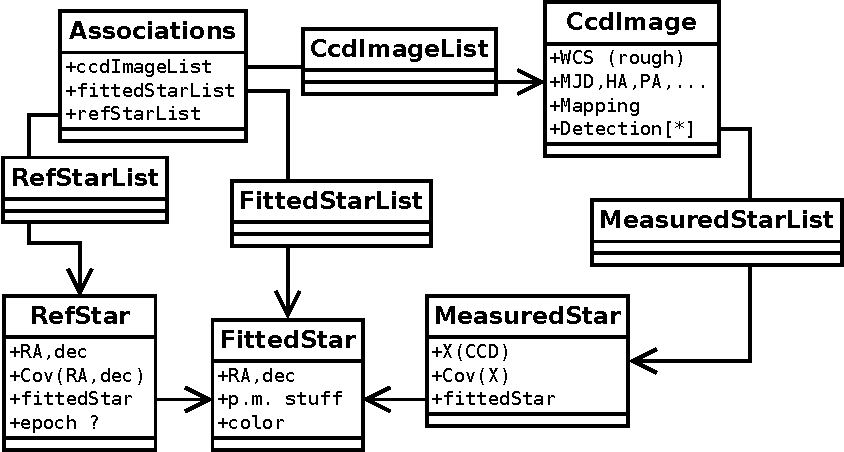
\includegraphics[width=0.8\textwidth]{_static/AssocClasses}
\caption{Chart of class relations which implement the associations between
input catalogs. One \class{FittedStar} usually has several \class{MeasuredStar}
pointing to it, and each \class{RefStar} points to exactly one \class{FittedStar}.
Most \class{FittedStar}'s have no \class{RefStar}. \label{fig:AssocClasses} }
\end{figure}

The \class{Associations} class holds the list of input \class{CcdImage}'s
and connects together the measurements of the same object. The input
measurements are called \class{MeasuredStar} and the common detections
are called \class{FittedStar}. The objects collected in an external
catalog are called \class{RefStar}. Despite their names, these classes
can represent galaxies as well as stars. The collections of sush objects
are stored into \class{MeasuredStarList}, \class{RefStarList} and
\class{FittedStarList}, which are container derived from \class{std::list}.
The relations between these classes, all implemented in C++, are displayed
in \prettyref{fig:AssocClasses}.

\section{Fitting the transformations between a set of images}

Some applications require determination of transformations between
images rather than mappings on the sky. For example a simultaneous
fit of PSF photometry for the computation of the light curve a point-like
transient requires mappings between images to transport the common
position in pixel space from some reference image to any other in
the series. The calexp series would typically involve the CCD from
each exposure that covers the region of interest. The package described
here can fit for the needed mappings: 
\begin{itemize}
\item in order to remove all reference terms from the $\chi^{2}$ of eq.
\prettyref{eq:astrometry-chi2}, one avoids calling \method{Associations::CollectRefStars}. 
\item One chooses polynomial mappings for all Calexp except, reserving one
to serve as a reference with a fixed identity mapping. The distortion
model \class{SimplePolyModel} allows that. 
\item Chose identity projectors (the class \class{IdentityProjector} does
precisely that). 
\end{itemize}
So, fitting transformations between image sets can be done with the
provided code.

\appendix

\section{Representation of distortions in SIP WCS's \label{sec:sip-wcs}}

The purpose of the appendix is to provide the minimal introduction
to WCS concepts required to understand the code (and the comments)
when browsing through it. Readers familiar with WCSs can give up here.

WCS's are abstract concepts meant to map data on coordinate systems.
In the astronomical imaging framework, this almost always means mapping
the pixel space into sidereal coordinates, expressed in some conventional
space\footnote{The WCS concepts are broad enough to accommodate mapping of planet
images, but we will obviously not venture into that.}. One key aspect of the WCS ``system'' is that it proposes some
implementation of the mappings in FITS headers, which comes with software
libraries to decode and encode the mappings. The WCS conventions cover
a very broad scope of applications, and wide-field imaging makes use
of a very small subset of those.

For the mappings used in wide-field imaging, the transformation from
pixel space to sky can be pictured in two steps: 
\begin{enumerate}
\item mapping coordinates in pixel space onto a plane. 
\item de-projecting this plane to the celestial sphere. 
\end{enumerate}
Let us clear up the projection/de-projection step first. There are
plenty of choices possible here, and the differences only matter fir
really large images. The projection used by default in the imaging
community seems to be the gnomonic projection: the intermediate space
is a plane tangent to the celestial sphere and the plane$\rightarrow$sphere
correspondence is obtained by drawing lines that go through the center
of the sphere. In practice there is no need to know that, because
any software dealing with WCS's can pick up the right FITS keywords
and compute the required projection and de-projection. For this gnomonic
projection, one finds \verb&CTYPE1='RA---TAN'& and \verb&CTYPE2='DEC--TAN'&
in the FITS header. This projection is often used to generate re-sampled
and/or co-added images and one should keep in mind that, for large
images, the pixels are not exactly iso-area. One point of convention
that might be useful to keep in mind; is that WCS conventions express
angles in degrees. In the gnomonic projection, offsets in the tangent
plane are expressed in degrees (defined through angles along great
circles at the tangent point), so that the metric in the tangent plane
is ortho-normal), and sidereal angles evaluated on the sky are also
provided in degrees by the standard implementations. A notable exception
is the LSST software stack where, by default, the angles are provided
in radians.

We now come back to the first mapping step, i.e. converting coordinates
measured in pixel units into some intermediate coordinate system.
The universal WCS convention here is pretty minimal: it allows for
an affine transform, which is in general not sufficient to map the
optical distortions of the imaging system, even after a clever choice
of the projection. Extensions of the WCS convention have been proposed
here, but none is universally understood. The LSST software stack
implements the SIP addition, which consists in applying a 2-d polynomial
transform to the CCD space coordinates, prior to entering the standard
WCS chain (affine transform, then de-projection). In practice, the
SIP ``twisting'' is applied by the LSST software itself (in the
class \class{afw::image::TanWcs}), and the ``standard'' part (affine
and de-projection, or the reverse transform) are sub-contracted to
the ``libwcs'' code.

One common complication of the WCS arena is that it was designed in
the FITS framework convention, itself highly Fortran-biased for array
indexing, so that the first corner pixel of an image is indexed (1,1).
The LSST software, and most modern environments use C-like indexing,
i.e. images stars at (0,0), as well as coordinates in images. The
WCS LSST software hides this detail to users, by offsetting the pixel
space coordinates provided and obtained from the wcs-handling library.

We now detail what is involved in the SIP convention: the SIP ``twisting''
itself is encoded through 4 polynomials of 2 variables, which encode
the direct and reverse transformations. The standard affine transform
is expressed through a $2\times2$ matrix ($Cd$) and a reference
point $X_{ref}$ (called \verb'CRPIX' in the fits header): 
\[
Y_{TP}=Cd(X_{pix}-X_{ref})
\]
$X_{pix}$ is a point in the CCD space, and $Y_{TP}$ is its transform
in the tangent plane. Obviously, $X_{pix}$ and $X_{ref}$ should
be expressed in the same frame so that the transform does not depend
this frame choice. We write symbolically this transform as $Y_{TP}=L(X_{pix})$
The SIP distortions are defined by a polynomial transformation in
pixel space, that we call $P_{A}$, for the forward transformation.
By convention, the transform from pixel space to tangent plane then
reads: 
\[
Y_{TP}=L\left(X_{pix}-X_{ref}+P_{A}(X_{pix}-X_{ref})\right)
\]
which again does not depend on the frame choice (0-based or 1-based),
provided $X_{pix}$ and $X_{ref}$ are expressed in the same frame.

In \code{jointcal} ,the internal representation of SIP WCS's uses
three straight 2d$\rightarrow$2d transformations: the SIP correction,
the affine transformation and the de-projection. Those are just composed
to yield the actual transform, and the two first ones are generic
polynomial transformations. We provide routines to translate the TanWcs
objects into our representation (\method{ConvertTanWcs}) and back
(\method{GtransfoToTanWcs}). In the latter case, we also derive the
reverse distortion polynomials, which are built if needed in our representation
of SIP WCSs.

\section{Notes on meas\_mosaic (from HSC)}

Naoki Yasuda wrote \emph{meas\_mosaic} for HSC processing, with a
similar goal as \code{jointcal}.

For photometry, \emph{meas\_mosaic }fits a 7th order Chebyshev polynomial
on the focal plane, plus a zeropoint offset per CCD. The polynomial
coefficients are written to the header of \textbf{fcr-{[}visit{]}-{[}ccd{]}.fits}
files as \textbf{C\_N\_M} values, while the zeropoint and its error
is written as \textbf{FLUXMAG0} and \textbf{FLUXMAG0ERR}. That calibration
is applied to all of the fluxes in the catalog, which are written
out to the same ``\emph{{*}\_flux}'' catalog fields (converting
them to magnitudes in the process).

\bibliography{lsst,lsst-dm,refs,refs_ads,books,jointcal}

\end{document}
